
\documentclass[a4paper,12pt]{article}
\usepackage{acn-scientific}
\usetikzlibrary{decorations.pathreplacing,
  decorations.markings,
  decorations.pathmorphing}
\usetikzlibrary{patterns,fadings}

\setcounter{secnumdepth}{0}

%\addtolength{\voffset}{-2cm}
%\addtolength{\textheight}{4cm}

%\title{AQA Unit PHYA1\\Particles, Quantum Phenomena and Electricity}
\title{AQA Unit PHYA1\\Electromagnetic~Radiation and Quantum~Phenomena}
\author{Mr \textsc{A.C. Norman}\\
\textsc{Bishop Heber High School}
\\ \texttt{anorman@bishopheber.cheshire.sch.uk}}
\date{Autumn Term, 2012}

\begin{document}
\begin{titlepage}
\maketitle

\thispagestyle{empty}
\enlargethispage{4cm}
	
\noindent\includegraphics[width=\textwidth]{img/photon.jpg}

\footnotesize
\begin{quotation}
This sequence of photographs shows that photography is a quantum process. In the fist photographs, the number of photons is very small, and they arrive on the film with a probability proportional to the brightness of the image at that point. The number of photons ranges from about 3 000 in the first exposure to about 30 000 000 in the final exposure 
\end{quotation}
\begin{flushright}
[CREDIT: Prof. Thomas D. Rossing, \emph{Vision: Human and electronic}]
\end{flushright}

\normalsize

\end{titlepage}
\newpage

\thispagestyle{empty}
\addtocounter{page}{-1}

\begin{center}
\fbox{
\begin{minipage}{0.7\textwidth}
\vspace*{1em}
\begin{center}
\includegraphics[width=0.3\textwidth]{by-nc-sa.png}
\end{center}

This work is licensed under a Creative Commons
Attribution-NonCommercial-ShareAlike License.

{\footnotesize\texttt{http://creativecommons.org/licenses/by-nc-sa/3.0/}}\\

Non-commercial uses are thus permitted without any
further permission from the copyright owner.\\

%Permissions beyond the scope of this license are
%administered by the author. Information on how
%to request permission may be found at:
%http://www.randomhouse.com/about/
%permissions.html
\end{minipage}
}
\end{center}

%\tableofcontents
\clearpage
%\part{Waves}

%CONTENT:

\section{The photoelectric effect}

Sometimes, visible or ultra-violet light falling on a metal surface can cause electrons to be emitted from the metal.  For most metals, ultra-violet light is needed, but some metals will exhibit this phenomenon with visible light, e.g.\ sodium will emit electons with green light\footnote{This works with visible light for the other alkali metals too, and there are even semi-conductors with special coatings that will emit electrons all the way through the visible spectrum and into the infra-red.}.  This phenomenon is known as the \emph{photoelectric effect}.

Metals have high electrical conductivity, and usually one or two electrons per atom are free to move about, termed the `conduction electrons'. We can grasp how metals are bonded together by thinking of a regular structure of positive ions with the conduction electrons moving about in between, creating a more-or-less uniform sea of negative charge which glues the structure together.  Light cannot turn into electrons (charge must be conserved!) so the light must be giving electrons in the metal enough energy to escape from the electrostatic attraction of the metal nuclei.

%diagram
\begin{center}
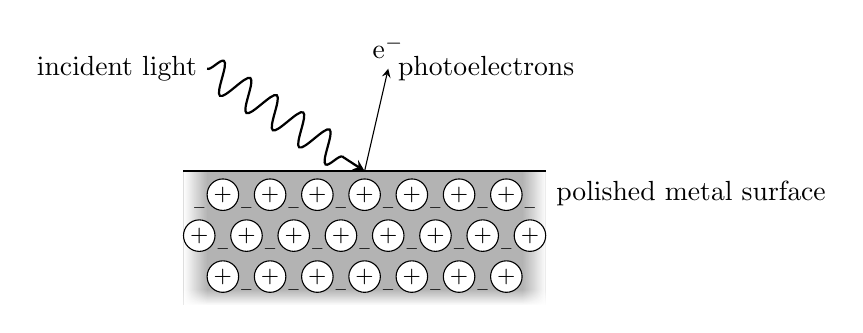
\begin{tikzpicture}[
lightray/.style={thick,>=stealth,->,decorate, decoration={snake,post length=3mm,amplitude=2mm,segment length=4mm}}]
% interface
\fill[fill=gray,opacity=0.6] (-0.3,0)--(4.3,0)--(4.3,-1.7)--(-0.3,-1.7)--(-0.3,0);
\begin{scope}[transparency group]
        % Left edge
        \fill[path fading=east, color=white] (-0.3,-1.7) rectangle (0,0);
        % Bottom edge
        \fill[path fading=north, color=white] (-0.3,-1.7) rectangle (4.3,-1.5);
        % Right edge
        \fill[path fading=west, color=white] (4.0,-1.7) rectangle (4.3,0);
    \end{scope}
\draw[line width=1pt] (-0.3,0)-- (4.3,0)node[anchor=north west]{polished metal surface};
% +ve ions
\foreach \i in {0.2,0.8,...,4.0}{
\draw[fill=white] (\i,-0.3) node{\footnotesize $+$} circle (0.2);
\draw[fill=white] (\i+0.3,-0.8196) node{\footnotesize $+$} circle (0.2);
\draw[fill=white] (\i,-1.34) node{\footnotesize $+$} circle (0.2);
}
\draw[fill=white] (-0.1,-0.82) node{\footnotesize $+$} circle (0.2);
% -ve charges in cloud NB important to have same number of + and -
\foreach \j in {0.2,0.8,...,3.8}{
\node at (\j+0.3,-0.473) {\tiny $-$};
\node at (\j,-0.9928) {\tiny $-$};
\node at (\j+0.3,-1.5124) {\tiny $-$};
}
\node at (4.1,-0.473) {\tiny $-$};
\node at (-0.1,-0.473) {\tiny $-$};
\node at (3.8,-0.9928) {\tiny $-$};
%light rays
\draw[lightray] (0,1.3)node[left]{incident light}--(2,0);
\draw[>=stealth,->] (2,0)--(2.3,1.3)node[right]{photoelectrons}node[anchor=south]{$\mathrm{e}^{-}$};
\end{tikzpicture}
\end{center}


The classical picture of light as a wave would explain the photoelectric emission of electrons as a result of the electrons gaining enough energy to escape the metal surface from being shaken about by the light wave tossing it around (like a boat on the sea).\footnote{The `water' here is the electric and magnetic fields---an electromagnetic wave is a disturbance in these fields---and the electron is `tossed about' because it feels a changing force as these fields change, due to its charge.}  As the light is made brighter, these disturbances are greater, since the light has greater intensity and therefore the wave has a bigger amplitude.

However, Einstein realized in 1905 that this picture could not fully explain the experimental observations of the photoelectric effect.  In particular:
\begin{itemize}
\item as the light intensity is turned down, there is no threshold intensity below which no electrons are emitted: they continue being emitted (albeit less often) no matter how dim the light is, and indeed some may be emitted \emph{as soon as the light is turned on}!
\item as the light intensity is increased, the electrons which are emitted do not get more energetic.  There are more of them, but their (kinetic) energy remains the same.
\item if the frequency of the light is changed, there is a certain frequency below which no electrons will be emitted \emph{no matter how intense the light is made}.
\end{itemize}

This led Einstein to relate these results to Planck's hypothesis that matter can only accept or emit radiation energy in small packets \emph{quanta} of a definite size related to the frequency of the light by $E=hf$, where $E$ is the energy of the quantum, $f$ is the frequency of the light radiation and $h$ is a constant of proportionality known as \emph{Planck's constant},\footnote{Named after Max Planck (1858-1947), who resolved the `ultraviolet catastophe' of the experimental observations of black body radiation, and thus originated quantum theory.} equal to \SI{6.64e-34}{J.s}. He furthermore postulated that light comprises a finite number of individual packets of energy (which we now call \emph{photons}) which carry an energy $hf$ and transfer all their energy to the photoelectrons during a collision.\footnote{Einstein got a Nobel prize in 1921 ``for his services to theoretical physics, and especially for his discovery of the law of the photoelectric effect''.}

The photoelectrons emitted from the metal surface need a certain minimum energy to escape from the metal, known as the \emph{work function} $\phi$, so the minimum or threshold frequency $f_{0}$ of photon that can give rise to photoelectrons must have this energy $hf_{0}=\phi$.

The kinetic energy $\frac{1}{2}m_{\mathrm{e}}v^2$ of a photoelectron leaving the metal surface also comes from the energy given to it by the photon that it absorbed: any extra energy above the minimum required that the incoming photon has---once the energy of the work function has been used to escape from the metal---goes into the photoelecton's kinetic energy:

\[\frac{1}{2}m_{\mathrm{e}}v^2=hf-\phi.\]

%EXAMPLES OF EQUATION??

In this way, Einstein was able to explain all of the experimental results in a simple theory, and his equation for the kinetic energy above was verified experimentally in 1912,\footnote{Following the publication for an accurate value for the mass of the electron produced by using Millikan's oil drop experiment and earlier measurements of the electron specific charge.} but one which was at odds with the many other extremely wide ranging experiments which had lead scientists to the conclusion that light is a form of wave motion.  This idea therefore had been overturned---there is no way to explain the experimental facts using it---and the decades that followed rewrote the whole of physics, in what became known as `the quantum revolution'.


\section{Collisions of electrons with atoms}

When electrons collide with atoms, what happens depends on the speed (and therefore the kinetic energy) of the electron.  At very low energies, the electron will collide elastically with the atoms, i.e.\ they will bounce off without losing any energy.  As the energy is increased, inelastic collisions start to occur, and the electrons stand a chance of losing energy to the atom, changing its internal arrangement in the process.

\subsection{Ionization}

An ion is a charged atom, one which has gained or lost one (or more) electrons, so that the number of electrons no longer equals the number of protons, as it does in a neutral atom.  We have already seen that in a metal, most of the atoms have at least one electron which can move freely around the metal, leaving them as positive ions.  Atoms can become ionized by gaining or losing electrons in lots of different ways, including chemical bonding (and in particular ionic bonding); having their electrons knocked out by passing alpha or beta particles from radioactive substances; decaying radioactively themselves by $\alpha$ or $\beta$ decay; having their electrons annihilated by positrons; or being subjected to a too strong electric or magnetic fields.

A \emph{plasma} is any ionized gas: a gas made up partly or completely of charged particles like ions\footnote{Most astrophysicists think that 99.9\% of all observable matter is in the form of plasma.}.  We most often encounter such a gas when electrons pass through a gas, with enough energy to knock electrons out of the gas atoms and make them into ions.

The energies required are often measured using the unit of the electron volt (\si{eV}).\footnote{An electron volt (\si{eV}) is equal to the energy an electron has gained when it has moved through a potential difference of one volt.  Since the work done when a particle of charge $Q$ moves through a potential $V$ is $E=QV$, an electron which has a charge of \SI{1.6e-19}{C} will gain \SI{1.6e-19}{J} of (kinetic) energy when it is accelerated through a p.d. of \SI{1}{V}.}  At first this may seem an odd unit of energy to use, compared to the \si{J} with which you are more familiar, but it is just the right size and is therefore most useful when dealing with energies on an atomic scale.

\[\SI{1}{eV}=\SI{1.6e-19}{J}.\]

The minimum amount of energy that is needed to ionize an atom (i.e.\ to remove its most loosely bound electron) is known as the \emph{ionization energy}.  For example, the ionization energy of hydrogen is \SI{13.6}{eV} (or \SI{2.18e-18}{J}).  Of course, hydrogen only has one electron, but for other elements, we could go on removing electrons.  The energy needed to remove the next most loosely bound electron is called the second ionization energy, and so on\ldots

We can see from the definition of the electron volt that \SI{13.6}{eV} is the kinetic energy gained by an electron when it is accelerated through a p.d. of \SI{13.6}{V}.  Therefore, if an electron which has been accelerated from rest through a p.d. of \SI{13.6}{eV} or more collides with a hydrogen atom, it has enough energy to knock the hydrogen's electron out of the atom and leave the hydrogen ionized.  This in fact is a common way to produce ionized gases in the laboratory, via a low pressure gas between electrodes in a long narrow glass tube, and such an arrangement is known as a discharge tube.  The ionized gas glows a characteristic colour, for reasons we shall discover when we discuss line spectra. %section \ref{photon-emission}.

\subsection{Excitation}

Gas atoms can still absorb energy from electrons without being ionized.  In fact, even if the incoming electron does not have enough energy to completely remove an electron (and the easiest electron to remove is the most loosely bound one), it might be able to `excite' the atom by giving one of its electrons some energy.  The excited electron can then move into a higher energy state (one which is further from the nucleus).

For example, the first and second \emph{excitation energies} of hydrogen are \SI{10.2}{eV} and \SI{12.1}{eV} respectively.  An energetic incoming electron striking a hydrogen atom might bounce off elastically, losing no energy; it might excite the hydrogen atom, losing one of these amounts of energy doing so; or it might ionize the hydrogen atom completely, losing \SI{13.6}{eV} of energy.  There will be a certain probability of each occurring.
%check this Calculation of the 1s-2s Electron Excitation Cross Section of Hydrogen 1958 Proc. Phys. Soc. 72 121 Excitation by electron collision of excited atomic hydrogen K Omidvar - Physical Review, 1965 - APS J. Phys. Chem. Ref. Data 19, 617 (1990); http://dx.doi.org/10.1063/1.555856 (20 pages) Cross Sections and Related Data for Electron Collisions with Hydrogen Molecules and Molecular Ions


\section{Energy levels and photon emission}

The energy of an electron which is confined in an atom can have only certain values, called the \emph{energy levels} of the atom.  The energy levels of an atom of a particular element are different from those of all other elements, and are the same for any atom of that element.

The following diagram represents the energy levels of a hydrogen atom.  Hydrogen's only electron is normally in the lowest energy level, which has an energy of \SI{-13.6}{eV},\footnote{The energy levels are defined with reference to an electron which is free from the influence of the nucleus (i.e.\ it has been ionized), which is taken as having zero energy.  This is why all of the energy levels have negative energy.} and when it is there the atom is said to be in its \emph{ground state}.

If a hydrogen atom absorbs energy in some way (for example by being hit by an electron or a photon), its electron may be promoted to one of the higher energy levels.  The atom is now unstable---the electron could randomly fall back down to the lowest level at any time---and is in what is called an \emph{excited state}.  \emph{Deexcitation} is the name given to the process whereby the atom returns to its ground state again, and the energy that the electron has loses in returning to this lower energy state is emitted as light (in fact as a single photon of exactly the right frequency to have this energy).

\begin{figure}
  \begin{tikzpicture}[scale=0.6]
    %\draw (0,0) -- (6,0);
    \newcounter{j}
    \foreach \i in {1,2,...,4}{
      \draw  (0,-13.6/\i/\i)node[left] {\footnotesize$n=\i$} -- (10,-13.6/\i/\i);  
    }
    \foreach \i in {5,6,...,99}{
      \draw  (0,-13.6/\i/\i) -- (10,-13.6/\i/\i);
    }
 \draw (10,-13.6)node[right]{\footnotesize$-13.6$}
  (10,-13.6/4)node[right]{\footnotesize$-3.40$}
  (10,-13.6/9)node[right]{\footnotesize$-1.51$}
  (10,-13.6/16)node[right]{\footnotesize$-0.85$};
    \draw  (0,-13.6/10000)node[left] {\footnotesize$n=\infty$} -- (10,-13.6/10000)node[right]{\footnotesize zero};
  \draw[>=stealth,->] (12,-11)--node[right]{Energy in \si{eV}}(12,-5);
  \draw[->] (14,-13.6) node[right]{ground state}--(12,-13.6);
    \draw[->] (14,-13.6/9) node[right]{an excited state}--(12,-13.6/9);
    \draw[->] (14,-13.6/10000) node[right]{free electron (ionized)}--(12,-13.6/10000);
  \end{tikzpicture}
\end{figure}

\label{photon-emission}

Let us imagine that an electron in a hydrogen atom has somehow been excited into the $n=4$ energy level.  After a short time, it will return to the $n=1$ energy level, but it has four possible routes to this ground state:
\[n=4 \;\longrightarrow\; n=3 \; \;\longrightarrow\; n=2 \;\longrightarrow\; n=1,\]
\[n=4 \;\longrightarrow\; n=3 \;\longrightarrow\; n=1,\]
\[n=4 \;\longrightarrow\; n=2 \;\longrightarrow\; n=1,\]
\[n=4 \;\longrightarrow\; n=1.\]

This actually involves six different transitions: $n=4\rightarrow3$,$4\rightarrow2$,$4\rightarrow1$,$3\rightarrow2$,$3\rightarrow1$,$2\rightarrow1$, each of which will involve the emission of a photon whose frequency depends on the difference in energy between the levels involved.  When an electron moves from a level with energy $E_{2}$ to one of lower energy $E_{1}$, the frequency $f$ of the emitted photon is given by the difference in energies:
\[hf=E_{1}-E_{2}.\]

\begin{marginfigure}
\includegraphics[width=\textwidth]{img/neon.jpg}
\caption{Part of the line spectrum of neon, created using a low pressure glass discharge tube and viewed via a diffraction grating spectrometer at Bishop Heber High School.}
\end{marginfigure}

Where there are lots of atoms, all possible transitions can be expected to occur in even a very short time interval, and photons of many different specific frequencies are emitted.  The line spectrum of hydrogen is thus composed of light of the frequencies of all the transitions above (and many more besides).  This is why discharge tubes, in which electricity is passed through a low pressure gas allowing electrons to excite atoms in the gas, are seen to glow with a colour distinctive colour depending on the gas inside, and the lines in the spectrum---corresponding to the transitions between atomic energy levels---are characteristic of the element.  This is how we can know the composition of far-off stars and planets.\footnote{Though in these cases it is usually by absorption spectra, i.e.\ dark lines in a continuous spectrum which correspond to the positions of the spectral lines of the excited elements.}


\section{Fluorescence}

It is possible that an atom which has been excited by absorbing a photon will not return to its initial state by emitting a photon of the same energy, but will instead go to an interim state for a time and emit a photon of lower energy than the photon which was originally absorbed.

This ability to seemingly change the wavelength of light (absorbing at one wavelength and emitting light of another wavelength) was known about and studied long before quantum theory was developed.  If the light is emitted rapidly following absorption, the process is called \emph{fluorescence},\marginnote{George Gabriel Stokes coined this term in his 1852 paper on the ``Refrangibility'' (wavelength change) of light, after studying extensively the ability of fluorspar and uranium glass to change invisible light beyond the violet end of the visible spectrum into blue light. He wrote ``I am almost inclined to coin a word, and call the appearance fluorescence, from fluor-spar [i.e.\ fluorite]''.} whereas if there is an appreciable delay (in some cases seconds, minutes or even many hours) it is called \emph{phosphorescence}.

The most striking examples of fluorescence occur when the absorbed radiation is in the ultraviolet region of the spectrum, and thus invisible to the human eye, and the emitted light is in the visible region.  Any number of commonplace materials (e.g.\ detergents, organic dyes, tonic water, and tooth enamel) will emit characteristic visible photons so that they appear to glow under ultraviolet illumination.

\begin{figure}
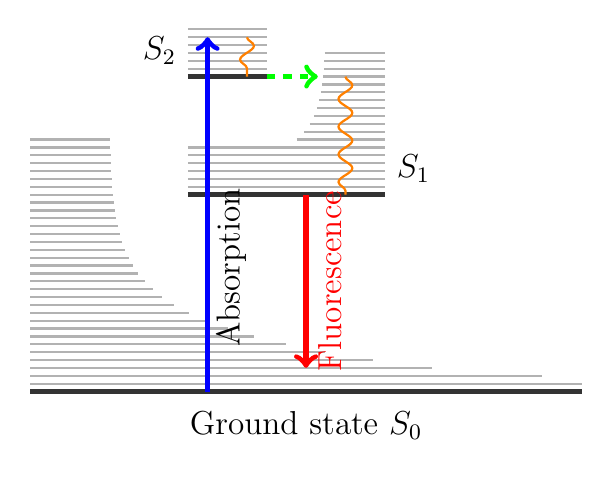
\begin{tikzpicture}[scale=0.5]

    % styles
    \tikzstyle{elec} = [line width=2pt,draw=black!80]
    \tikzstyle{vib} = [thick,draw=black!30]
    \tikzstyle{trans} = [line width=2pt,->]
    \tikzstyle{transCI} = [trans,dashed,draw=green]
    \tikzstyle{relax} = [draw=orange,thick,decorate,decoration=snake]
    \tikzstyle{rv} = [rotate=90,text=orange,pos=0.5,yshift=3mm]

    % fundamental
    \path[elec] (0,0)  -- ++ (14,0)
        node[below,pos=0.5,yshift=-1mm] {\large Ground state $S_0$};
    \path[vib] (0,0.2) -- ++ (14,0);
    \path[vib] (0,0.4) -- ++ (13,0);
    \foreach \i in {1,2,...,30} {
        \path[vib] (0,0.4 + \i*0.2) -- ++ ({2 + 10*exp(-0.2*\i)},0);
    }

    % S1
    \path[elec] (4,5) -- ++ (5,0)node[anchor=south west] {\large $S_1$};
    \foreach \i in {1,2,...,6} {
        \path[vib] (4,5 + \i*0.2) -- ++ (5,0);
    }
    \foreach \i in {1,2,...,12} {
        \path[vib] ({7.5 - 1*exp(-0.3*\i)},6.2+\i*0.2) -- (9,6.2+\i*0.2);
    }

    % S2
    \path[elec] (4,8) node[anchor=south east] {\large $S_2$} -- ++ (2,0);
    \foreach \i in {1,2,...,6} {
        \path[vib] (4,8 + \i*0.2) -- ++ (2,0);
    }

    % absorption
    \path[trans,draw=blue] (4.5,0) -- ++(0,9)
        node[rotate=90,pos=0.35,text=black,yshift=-3mm] {\large Absorption};

    % fluo
        \path[trans,draw=red](7,5) -- ++(0,-4.4)
        node[rotate=90,pos=0.5,text=red,yshift=-3mm] {\large Fluorescence};
        
        %IC
        \path[transCI] (6,8) -- ++(1.3,0);

    % relaxation vib
    \path[relax] (5.5,9.0) -- ++(0,-1.0);
    \path[relax] (8,8)     -- ++(0,-3);
\end{tikzpicture}
\caption{A Jablonski diagram showing fluorescence occuring via the closely spaced energy levels in a molecule.}
\end{figure}

There is widespread commercial use of fluorescent substances, for example in washing powders and paper to `whiten' (making white bluer makes it appear a crisper, whiter white).  Highlighter ink is often fluorescent due to the presence of pyranine.  Banknotes, postage stamps and credit cards also often have fluorescent security features.

\subsection{Fluorescent tube}
The common fluorescent lamp relies on fluorescence to convert the invisible ultraviolet radiation emitted by a mercury discharge tube into visible light.  The inside of the glass of the discharge tube is coated with fluorescent phosphors which absorbs ultraviolet and re-emits visible light.

The low pressure mercury within the tube of a fluorescent lamp has an emission spectrum (the emission is caused by electrons hitting the gaseous mercury atoms when electricity is passed through the tube) which is dominated by a line in the ultraviolet at \SI{254}{nm}, which is converted into visible emissions at many different wavelengths in the visible spectrum by the phosphors.

\begin{figure}
  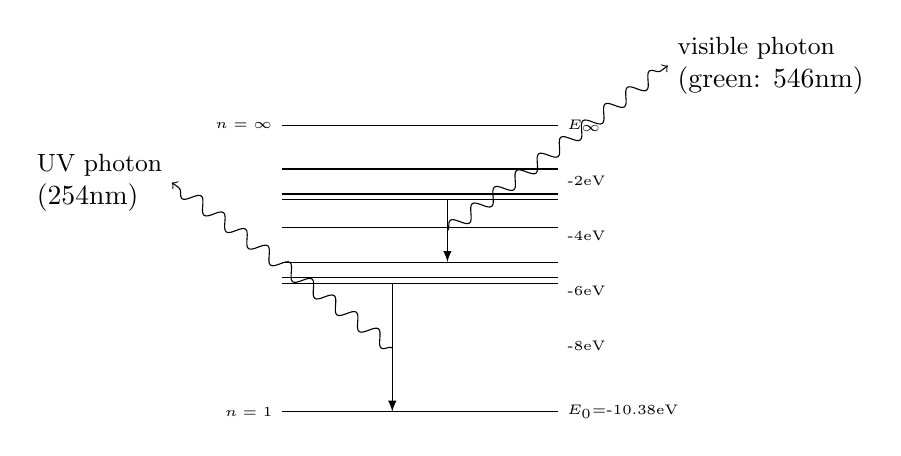
\begin{tikzpicture}[scale=0.35]
  %\draw (0,0) -- (6,0);
  \foreach \i in {-1.56,-1.57,-2.48,-2.68,-3.71,-4.95,-5.52,-5.74}{
  \draw  (0,\i) -- (10,\i);
  }
  \draw  (0,-10.38)node[left] {\tiny$n=1$} -- (10,-10.38)node[right]{\tiny$E_{0}$=\SI{-10.38}{eV}};
  \draw  (0,0)node[left] {\tiny$n=\infty$} -- (10,0)node[right]{\tiny$E_{\infty}$};
  \draw  (10,-2) node[right]{\tiny\SI{-2}{eV}};
  \draw  (10,-4) node[right]{\tiny\SI{-4}{eV}};
  \draw  (10,-6) node[right]{\tiny\SI{-6}{eV}};
  \draw  (10,-8) node[right]{\tiny\SI{-8}{eV}};
  %UV photon
  \draw[>=latex,->] (4,-5.74) --(4,-10.38);
  \draw[decorate, decoration={snake},->] (4,-8.06)--++(-8,6)node[left,align=left]{\small UV photon\\(\SI{254}{nm})};
  %Vis photon
  \draw[>=latex,->] (6,-2.68) --(6,-4.95);
  \draw[decorate, decoration={snake},->] (6,-3.82)--++(8,6)node[right,align=left]{\small visible photon\\(green: \SI{546}{nm})};
  \end{tikzpicture}
\caption{Energy levels within the mercury atom.  Two transitions, giving rise to a visible and a UV photon respectively, are shown.}
\end{figure}

Mercury also emits visible light at wavelengths of \SI{436}{nm} (blue), \SI{546}{nm} (green), and \SI{579}{nm} (yellow-orange).  These three lines can be observed superimposed on the white continuous spectrum by using a spectroscope, or even when looking at the spectrum diffracted from a CD.

\begin{marginfigure}
\includegraphics[width=\textwidth]{img/cfl.jpg}
\caption{Part of the line spectrum of a compact fluorescent tube, viewed via a diffraction grating spectrometer at Bishop Heber High School.}
\end{marginfigure}

Fluorescent lighting is more energy-efficient than old-fashioned incandescent bulbs (in which most of the input power gets turned into heat, not light).  A fluorescent tube can produce an equal amount of light using one quarter of the power of a filament bulb.  However, the uneven spectrum of traditional fluorescent lamps may cause certain colors to appear different than when illuminated by incandescent light or daylight.




\section{Wave-particle duality}
We have seen some phenomena, e.g.\ refraction, which can be explained by thinking of light behaving as though it were a wave.  Other phenomena, such as the photoelectric effect, suggest that light comprises particles.\footnote{The human eye is a very good instrument: it takes only five or six photons to activate a nerve cell and send a message to the brain.  If we were evolved a little further so we could see ten times more sensitively, we shouldn't have to have this discussion: we should all have seen very dim light of one colour as a series of intermittent flashes of equal intensity, as the individual photons hit our retina.}  In fact it is useful in some circumstances to describe light---and here we don't mean just the light we can see, but all sections of the electromagnetic spectrum---as a wave and in others look upon it as consisting of particles; these are both useful models that can be applied to different situations.  We find a strong analogy here to the fable of the seven blind men who ran into an elephant.  One man felt the trunk and said ``the elephant is a rope''; another felt the leg and said ``the elephant is a tree,'' and so on.

In 1924, Louis de Broglie (1892--1987) suggested that if light (being normally though of as a wave) can be thought of as particle, then things which we usually consider to be particles may have wavelike properties.  If a `particle' acts like a `wave' then it must have an associated wavelength.  This wavelength, de Broglie postulated, would be related to the momentum $p$ of a particle by
\[\lambda=\frac{h}{p}=\frac{h}{mv},\]
where $h$ is Planck's constant, and the wavelength $\lambda$ became known as the \emph{de Broglie wavelength}.

\subsection{Evidence supporting de Broglie's hypothesis}
The first evidence in support of this came in 1927 when electron diffraction was observed by two separate teams of scientists, George Paget Thomson (who passed a beam of electrons through a thin metal film) at the University of Aberdeen, and Clinton Davisson and Lester Germer (who sent an electron beam through a crystalline grid) at Bell Labs in the US.  This led to de Broglie being awarded the Nobel Prize for Physics in 1929 for his hypothesis. Thomson and Davisson shared the Nobel Prize for Physics in 1937 for their experimental work.

Davisson and Germer diffracted electrons from the surface of a nickel crystal.  They accelerated electrons through a high voltage, and fired them at the crystal observing the reflected electrons. They observed a diffraction pattern as the planes of the crystal act like a diffraction grating.  In their experiment, Davisson and Germer used \SI{5000}{V} to accelerate the electrons, giving a de Broglie wavelength of \SI{1.7e-11}{m} (this is equivalent to an X-ray wavelength for light, so the electrons should behave similarly to X-rays).\footnote{The electrons are given their kinetic energy by the accelerating voltage, so $\frac{1}{2}m_{e}v^{2}=eV$ or, rearranging, $mv=\sqrt{2m_{e}eV}$.  This allows us to determine the de Broglie wavelength $\lambda=\frac{h}{mv}=\frac{h}{\sqrt{2m_{e}eV}}=\SI{1.7e-11}{m}$.}  Since this wavelength is approximately equal to the crystal plane spacing, diffraction occurs.

Since these early particle diffraction experiments, protons, neutrons, and hydrogen and helium atoms have been diffracted and thus shown to have wavelike properties.  Larger everyday objects (often termed `macroscopic') will not undergo diffraction as their wavelength turns out to be smaller that any possible diffraction setup (e.g.\ a snooker ball moving at \SI{1}{m.s^{-1}} has a wavelength of approximately \SI{e-33}{m}).

%\subsection{Double slit interference with electrons}

%If we were to perform a double slits type experiment using electrons rather than light, we would get a pattern very similar to that produced with light, with the fringes being thousands of time closer together.

%It is obvious to think that half of the electrons pass through S1 and half through S2 and that the interference between the two sets of electrons causes the pattern.  But, this is NOT what happens.
%	If we reduce the intensity of the electron beam, so that only one electron arrives at the slits at any one time, we still get the interference pattern, as long as the time is made long enough.  The diagram below shows what the film looks like as the pattern builds up. 


%What must happen is that  each electron passes through both slits and interferes with itself.  It is not possible to predict where an electron will go after passing through the slits, but only to give probabilities - it is most likely to go to a light area, and least likely to go to a dark area.
%	The idea of an electron passing through both slits at the same time is clearly not consistent with the idea of a particle, but is understandable if we accept that electrons act like a wave. However, if we watch the electrons passing through the slits, so we know which slit an electron has gone through (and therefore make it act like a particle), the interference pattern disappears. 

%	Wave particle duality means that neither the particle or wave model can be used to explain everything that light or matter does.  On a small scale, these models will only work in certain circumstances.  The best model available is quantum mechanics, which describes in abstract mathematics what is happening, and abandons any relation to a "physical" picture.

%Electrons are behaving like waves here.  This is an example of the so-called `wave--particle duality'.




\end{document}
